\documentclass[12pt,parskip]{komatufte}
\usepackage[subpreambles=false]{standalone}

%%%%%%%%%%%%%%%%%%%%%%%%%%%
% Silence warning messages
\usepackage{silence}
\WarningsOff[scrlayer-notecolumn]
\WarningsOff[biblatex]

%%%%%%%%%%%%%%%%%%%%
% Commenting

%\usepackage[author=Lyndon]{pdfcomment}
%\newcommand{\pdfcomment}[1]{} %ignore all comments

%\usepackage{todonotes}
%\newcommand{\pdfcomment}{\todo}


%%%%%%%%%%%%%%%%%%%%
% Tables
\usepackage{booktabs}

%%%%%%%%%%%%%%%%%%%
% Fonts
\usepackage{tgadventor} %sans
\usepackage{tgpagella}  %serif
\usepackage{inconsolata} %mono
\usepackage[T1]{fontenc}

\usepackage{microtype}
\usepackage[all]{nowidow}
%%%%%%%%%%%%%%%%%%%%%%%
% Styling
\setcounter{secnumdepth}{4}
\setcounter{tocdepth}{2}

\usepackage{placeins}



%%%%%%%%%%%%%%%%%%%
% Math
\usepackage{amsmath, amssymb, stmaryrd, mathtools}
\DeclareMathOperator*{\argmin}{argmin}
\DeclareMathOperator*{\argmax}{argmax}

\usepackage{xparse,xstring,etoolbox}
% crossref this against notation section
\newcommand{\vv}[1]{\tilde{#1}} % vector
\newcommand{\seq}[1]{\mathcal{#1}} % sequence
\newcommand{\set}[1]{\mathbb{#1}} % set

%%%%%%%%%
% Indexing/sequence indexing
\newcommand{\seqind}[2]{#1^{#2}} % seqence index
\newcommand{\ind}[2]{#1_{#2}} % indexed
\newcommand{\disamb}[2]{#1^{\mathrm{#2}}} %disambiguated

%% Smart indexing and naming
\newcommand{\ifupper}[3]{
    \normalexpandarg
	\exploregroups
	\StrCount{ABCDEFGHIJKLMNOPQRSTUVWXYZ}{#1}[\uppercount]
	\ifnumgreater{\uppercount}{0}{#2}{#3}
}

%smart index
\DeclareDocumentCommand{\ii}{u{_} m}{
	\ifupper{#1}%
	{% just a single uppercase character, i.e. a matrix
		  %make sure the index is the right length
		\StrCount{#2}{,}[\indcount]
		\ifnumgreater{\indcount}{0}
		{ % Got multiple indexes so all good
		 	\ind{#1}{#2}
		}
		{ % Only 1 index so grab the column
		 	\ind{#1}{{:,#2}}
		}
	}%
	{% Not just a single upper case character
		\ind{#1}{#2}
	}
}

\DeclareDocumentCommand{\nn}{u{_} m}{
	\seqind{#1}{#2}
}

\DeclareDocumentCommand{\dd}{u{_} m}{
	\disamb{#1}{#2}
}

% Index of a vector
\DeclareDocumentCommand{\iv}{u{_} m}{\ii{\vv #1}_{#2}}
\DeclareDocumentCommand{\dv}{u{_} m}{\dd{\vv #1}_{#2}}
\DeclareDocumentCommand{\nv}{u{_} m}{\nn{\vv #1}_{#2}}

%exp
\let\oldexp\exp
\renewcommand{\exp}[1]{\oldexp \left( #1 \right)}
\newcommand{\exptwo}[1]{\oldexp_2 \left( #1 \right)}

\newcommand{\softmax}{\mathrm{smax}}

\DeclareMathOperator*{\expectedop}{\mathbb{E}}
\DeclareDocumentCommand{\expected}{u{_} m}{
	\expectedop\limits_{\mathrlap{#2}}
}

%%%%%%%%%%%%%%%%
%Graphics
\usepackage{tikz}
\usetikzlibrary{positioning, fit,  shapes.geometric}
\usepackage{ifthen}
\usepackage{etoolbox}

\tikzset{
	backgroundcolor/.style ={fill=white},
	every node/.append style={
		minimum height=7mm,
	},
	labe/.append style={
		%Blue,
		align = center,
		backgroundcolor,
		fill opacity=0.6,
		text opacity=1,
		font={\footnotesize\itshape}	
	},
	layer/.append style={
		draw,
		align = center,
		minimum height=7mm,
	},
	tight/.append style={
		inner sep=0.2mm,
	},
	lookupbox/.append style={
		draw=none,
		append after command={
		       	[shorten <= -0.5\pgflinewidth]
		       	([shift={(-1.5\pgflinewidth,-0.5\pgflinewidth)}]\tikzlastnode.north east)
		       	edge([shift={( 0.5\pgflinewidth,-0.5\pgflinewidth)}]\tikzlastnode.north west) 
		       	([shift={( 0.5\pgflinewidth,-0.5\pgflinewidth)}]\tikzlastnode.north west)
		       	edge([shift={( 0.5\pgflinewidth,-1.5\pgflinewidth)}]\tikzlastnode.south west)            
		       	([shift={( -1.5\pgflinewidth,+0.5\pgflinewidth)}]\tikzlastnode.south east)
		       	edge([shift={(-1.5\pgflinewidth,-0.5\pgflinewidth)}]\tikzlastnode.north east)
		},
		inner sep=0.7mm,
		outer sep=0mm,
		minimum width=25mm
	}
}

\usepackage{pgfplots}
\pgfplotsset{compat=1.14}
\pgfplotsset{sideplot/.append style={
		width=\notescolwidth,
		domain=-10:10,
		samples=101,
		smooth,
		enlarge y limits={abs=2},
		axis lines=middle,
		xlabel  = $z$,
		ylabel  = $y$,
	},
	equ/.append style={
		color=blue,
		thick,
		mark=none
	}
}

% Function  For a plot 
% it  needs to be declared in preamble because of how \makenote* interacts with multiple files
\def\errorsurface(#1,#2){(0.5*#1 + 0.7*#2 + sin(deg(1.5*#1 + #2^2)))^2}


\usepackage{graphicx}
\graphicspath{{./figs/}, {./}, {./figs/chaptersentencerrepr/}, {./figs/chapterintromachinelearning/}, {./figs/chapterwordrepr/}}
\usepackage{adjustbox}


%%%%%%%%%%%%%%%%%%%
% Refs
\usepackage{cleveref}

\addbibresource{master.bib}

%%%%%%%%%%%%%%%%%%%%
% Formatting

% for examples from natural language space.
\newcommand{\natlang}[1]{\ifmmode \text{``\texttt{#1}''} \else {``\texttt{#1}''}\fi}
% \ifmmode ``trick'' from https://tex.stackexchange.com/a/15194/5834

%%%%%%%%%%%%%%%%%%%%%

\begin{document}

\setchapterpreamble{%
	\dictum[the seven senses of \natlang{literally},
	 \textit{Oxford English Dictionary}, 3rd ed., 2011]
	{
		\begin{description}
			\setlength\itemsep{0em}
			\item[1a.] In a literal, exact, or actual sense; not figuratively, allegorically, etc.
			\item[1b.] Used to indicate that the following word or phrase must be taken in its literal sense, usually to add emphasis.
			\item[1c.] colloq. Used to indicate that some (frequently conventional) metaphorical or hyperbolical expression is to be taken in the strongest admissible sense: `virtually, as good as'; (also) `completely, utterly, absolutely' \ldots
			\item[2a ]With reference to a version of something, as a transcription, translation, etc.: in the very words, word for word.
			\item[2b.] In extended use. With exact fidelity of representation; faithfully.
			\item[3a.] With or by the letters (of a word). Obs. rare.
			\item[3b.] In or with regard to letters or literature. Obs. rare.
		\end{description}		
}}

\chapter{Word Sense Representations}\label{sec:word sense-representations}
\begin{abstract}
	In this chapter, techniques for representing the multiple meanings of a single word are discussed.
	This is a growing area, and is particularly important in languages where polysemous and homonymous words are common.
	This includes English, but it is even more prevalent in Mandarin for example.
	The techniques discussed can broadly be classified as lexical word sense representation,  and as word sense induction.
	The inductive techniques can be sub-classified as clustering-based or as prediction-based.
\end{abstract}
	
\section{Word Senses}

Words have multiple meanings.
A single representation for a word cannot truly describe the correct meaning in all contexts.
It may have some features that are applicable to some uses but not to others,
it may be an average of all features for all uses,
or it may only represent the most common sense.
For most word-embeddings it will be an unclear combination of all of the above.
Word sense embeddings attempt to find representations not of words, but of particular senses of words.




\aside[Polysemous/Homonymous]{A word with multiple meanings i.e. senses. For NLP representational purposes polysemous and homonymous are synonymous.}

\aside[Part of Speech/POS]{The syntactic category a word belongs to. Different POS tags come from different tag sets.
Can be simple as the WordNet tag set: noun, adjective, verb, etc. or complex as in the Brown tag set: VBG-\emph{verb, gerund/present participle}, NN-\emph{	noun, singular or mass}.
 }
\aside[Word-use]{An occurrence of a word in a text, such as a training corpus. Each word will have multiple uses in a text. Each word-use will only have one particular meaning and will thus belong to one synset.}
\aside[Lemma]{The base form of the word as defined by a lexicographical resource. It is normally closely related to (often identical to) the \emph{stem} which is the word's root form with all morphological inflections (e.g. tenses) removed.}
\aside[Lexeme]{The set of words that share a common lemma: \natlang{go}, \natlang{going}, \natlang{goes}, and \natlang{went} all belong to the lexeme headed by the lemma \natlang{go}}
\aside[Synset]{A synset is a set of synonymous words: that is words that have the same meaning. In lexographic terms the synset is the core unit of meaning. Identifying the synset of a word-use is the the same as identifying the word sense. Every word sense corresponds to one synset.}
\aside[Gloss]{A gloss is the dictionary entry for a word sense, it normally includes both the definition and an example of use.
In WordNet each synset shares a common gloss.}

%\aside[Sensekey]{This is not a commonly used phrase by linquists, but it is an important implementation detail when using WordNet for WSD tasks. It repressents the mapping between lemma+pos and synset, and is needed because that is a many-many relationship. It take the basic form \texttt{lemma\%pos\_id:lex\_filenum}}
\aside[Lemmatization]{Lemmatization is the method of converting a word into its lemma. Due to the similary of the lemma to the stem,  this in essence means removing the tense and plurality information (stemming), with some additional special-cases. WordNet is indexed by lemmas, and comes with a lemmatizer called morphy allowing any word to be looked up by lemmatizing it to it's lemma}
\aside[Unlemmatization]{Given lemma (as one can extract from WordNet) and a full POS tag (such as a Brown-style tag) for a word, it is possible to undo the lemmatization with a high degree of reliability using relatively simple rules (again due to the similarity of the lemma to the stem). The POS tag encodes the key inflectional features that are lost. Patten.en \pcite{de2012pattern} is a python library encoding such rules (pluralisation, verb conjugation, etc.); though combining them with the POS tag to drive them is a task left for the reader. This can be used to find substitute words using WordNet's features, for finding synonyms, antonyms and other lemmas from lexically related categories.}


The standard way to assign word senses is via some lexicographical resource, such as a dictionary, or a thesaurus.
There is not a canonical list of word senses that are consistently defined in English.
Every dictionary is unique, with different definitions and numbers of word senses.
The most commonly used lexicographical resource is WordNet \pcite{miller1995wordnet}, and the multi-lingual  BabelNet \pcite{navigli2010babelnet}.
The relationship between the terminology used in word sense problems is shown in \Cref{fig:wordsenseterms}


\begin{figure}
	\caption{The relationship between terms used to discuss various word sense problems.
		The lemma is used as the representation for the lexeme, for WordNet's purposes when indexing.
		For many tasks each the word-use is pre-tagged with its lemma and POS tag,
		as these can be found with high reliability using standard tools.
		Note that the arrows in this diagram are \emph{directional}.
		That is to say, for example, each Synset \emph{has 1} POS,
		but each POS \emph{has many} Synsets.
	}
	\label{fig:wordsenseterms}

	\resizebox{\textwidth}{!}{\begin{tikzpicture}[circle/.append style={draw, font=\footnotesize, rounded rectangle}]
		\node[circle](worduse){\normalsize Word-use\\ e.g.\\ \natlang{Fred \underline{goes} shopping}};
		\node[circle, above right = 2 of worduse](pos){\normalsize POS\\ e.g.\\ \emph{verb}};
		\node[circle, below right = 2 of worduse](lexeme){\normalsize Lexeme\\  e.g. \\ \{\natlang{go}, \natlang{going},\\ \natlang{goes}, \natlang{went}\}};
		\node[circle, draw, below right = 2 of pos](synset){\normalsize Synset\\ e.g. \\ \{\natlang{go}, \natlang{move}, \\ \natlang{locomote}\}};
		\node[circle, draw, left = 2 of lexeme](word){\normalsize Word\\ e.g. \\ \natlang{goes}};

		
		
		\draw[->] (worduse) edge node[labe] {has 1} (synset);
		\draw[->] (worduse) edge node[labe] {has 1} (pos);
		\draw[->] (worduse) edge node[labe] {has 1} (lexeme);
		\draw[->] (worduse) edge node[labe] {has 1} (word);
		
		\draw[->] (word) edge node[labe] {has 1} (lexeme);
		
		\draw[->] (synset) edge node[labe] {has 1} (pos);
		\draw[<->] (synset) edge node[labe] {has many} (lexeme);
		
		\node[circle, above right = 2 of synset](gloss){\normalsize Gloss\\ e.g. \\ \natlang{to change location \ldots}};
		\draw[<->] (synset) edge node[labe] {has 1} (gloss);
		
		\node[circle, right = 2 of lexeme](lemma){\normalsize Lemma\\ e.g. \\  \natlang{go}};
		\draw[<->] (lemma) edge node[labe] {has 1} (lexeme);
	\end{tikzpicture}}
	
	
\end{figure}



\subsection{Word Sense Disambiguation}
Word sense disambiguation is one of the hardest problems in NLP.
Very few systems significantly out perform the baseline, i.e. the most frequent sense (MFS) technique.

Progress on the problem is made difficult by several factors.

The sense is hard to identify from the context.
Determining the sense may require very long range information:
for example the information on context may not even be in the same sentence.
It may require knowing the domain of the text, because word sense uses vary between domains.
Such information is external to the text itself.
It may in-fact be intentionally unclear, with multiple correct interpretations, as in a pun.
It maybe unintentionally unknowable, due to a poor writing style, such that it would confuse any human reader.
These difficulties are compounded by the limited amount of data available.

There is only a relatively small amount of labelled data for word sense problems.
It is the general virtue of machine learning that given enough data, almost any input-output mapping problem (i.e. function approximation) can be solved.
Such an amount of word sense annotated data is not available.
This is in contrast to finding unsupervised word embeddings, which can be trained on any text that has ever been written.
The lack of very large scale training corpora renders fully supervised methods difficult.
It also results in small sized testing corpora; which leads to systems that may appear to perform well (on those small test corpora), but do not generalise to real world uses.
In addition, the lack of human agreement on the correct sense, resulting in weak ground truth, further makes creating new resources harder.
This limited amount of data compounds the problem's inherent difficulties.


It can also be said that word senses are highly artificial and do not adequately represent meaning.
However, WSD is required to interface with  lexicographical resources,
such as translation dictionaries (e.g. BabelNet), ontologies (e.g. OpenCyc), and other datasets (e.g. ImageNet \pcite{imagenet_cvpr09}).


It may be interesting to note, that the number of meanings that a word has is approximately inversely proportional related to its frequency of use rank \pcite{zipf1945meaning}.
That is to say the most common words have far more meanings than rarer words.
It is related to (and compounds with) the more well-known Zipf's Law on word use \pcite{zipf1949human}, and can similarly be explained-based on Zipf's core premise of the principle of least effort. 
This aligns well with our notion that precise (e.g. technical) words exist but are used only infrequently -- since they are only explaining a single situation.
This also means that by most word-uses are potentially very ambiguous.

The most commonly used word sense (for a given word) is also overwhelmingly more frequent than its less common brethren -- word sense usage also being roughly Zipfian distributed \pcite{Kilgarriff2004}.
For this reason the Most Frequent Sense (MFS) is a surprisingly hard baseline to beat in any WSD task.
\aside[Semantic Syllepsis]{
	(Also known as pathological sentences that kill almost all WSD systems.)
	Consider the sentence: \natlang{John used to work for the \emph{newspaper} that you are carrying.}.	In this sentence the word-use \natlang{newspaper} simultaneously have two different meanings: it is both the company, and the object.
	This violates our earlier statement that every word-use belongs to exactly one synset.
	WSD systems are unable to handle these sentences as they attempt to assign a single sense to each word-use.
	Most word sense induction systems cannot do much better: at best a new sense could be allocated for the joint use, which does not correspond to the linguistic notion of the word having two senses for different parts of the sentence.
	Most works on word sense disambiguation outright ignore these sentences, or consider them to be ungrammatical, or incorrect.
	However, they are readily understood and used without thought by most native speakers.
	These constructions are also known as \emph{zeugma}, although zeugma is itself a highly polysemous word, so its usage varies. 
}
\subsubsection{Most Frequent Sense}\label{sec:most-frequent-sense}
Given a sense annotated corpus, it is easy to count how often each sense of a word occurs.
Due to the over-whelming frequency of the most frequent sense, it is unlikely for even a small training corpus to have the most frequent sense differing from the use in the language as a whole.

The Most Frequent Sense (MFS) method of word sense disambiguation is defined by counting the frequency of a particular word sense for a particular POS tagged word.
For the $i$th word use being the word $\n w_i$, having some sense $\n s_j$
then without any further context the 
probability of that sense being the correct sense is $P(\n s_j \mid \n w_i)$.
One can use the part of speech tag $p_i$ (for the $i$th word use) as an additional condition, and thus find $P(\n s_j \mid \n w_i, p_i)$.
WordNet encodes this information for each lemma-synset pair (i.e. each word sense) using the SemCor corpus counts.
This is also used for sense ordering, which is why most frequent sense  is sometimes called first sense.
This is a readily available and practical method for getting a baseline probability of each sense.
Most frequent sense can be applied for word sense disambiguation using this frequency-based probability estimate:  $\argmax_{\forall \n s_j} P(\n s_j \mid \n w_i, p_i)$.


In the most recent SemEval WSD task \pcite{moro2015semeval},
MFS beat all submitted entries for English, both overall, and on almost all cuts of the data.
The results for other languages were not as good, however in other languages the true corpus-derived sense counts were not used.


\aside[WordNet is not a strong moral baseline]{
	WordNet, as a resource,-based partly on the work of Princeton undergraduate students in the early 1990's,
	and on the literature of 1961,
	is not the kind of resource one might hope for from an AI information perspective.
	
	The glosses include a number of biases.
	These biases are reflective of the language use, but are not necessarily ideal to be encoded into a system.
	For example: \natlang{\mbox{S: (v) nag}, peck, hen-peck (bother persistently with trivial complaints) `She nags her husband all day long's}.
	Other dictionaries regularly show up in the News for similar content.
	
	Another problem is the source of the word sense counts.
	As discussed in the main text, sense counts are important in WSD systems.
	The counts come from SemCor, a sense annotated subset of the Brown Corpus.
	The Brown Corpus is a sampling of American texts from 1961.
	The cultural norms of 1961 were not the norms of today.
	(For context, note that the US did not pass the Civil Rights act to end segregation until 1964).
	As such, one should not trust WordNet (or SemCor) to reflect current sense counts,
	for words which have undergone usage change since 1961.
	
	Furthermore, when creating down stream resources-based on WordNet,
	one should not use these sense counts to determine how important it is to include a concept.
	If ImageNet \parencite{imagenet_cvpr09} for example, had used SemCor counts to determine which synsets of images would be included,
	then items rarely discussed in 1961 literature, like  \natlang{wheelchairs}, and \natlang{prosthesis} would be excluded.
	Which would in turn make many image processing systems systematically unhelpful in processing images relating to the disabled.
	(Do not fear: even the initial release of ImageNet contains hundreds of images of \natlang{wheelchairs}, and \natlang{prosthesis})
	Unintentional biasing of data can have on-going effects on the behaviour of machine learning-based systems far beyond the original conception.
}

\section{Word Sense Representation}
It is desirable to create a vector representation of a word sense much like in \Cref{sec:word-representations} representations were created for words.
We desire to an embedding to represent each word sense, as normally represented by a word-synset pair.
This section considers the representations for the lexical word senses as given from a dictionary.
We consider a direct method of using a labelled corpus, and an indirect method makes use of simpler sense-embeddings to partially label a corpus before retraining.
These methods create representations corresponding to senses from WordNet.
\Cref{sec:word sense-induction-wsi} considers the case when the senses are to also be discovered, as well as represented.




\subsection{Directly supervised method}
The simple and direct method is to take a dataset that is annotated with word senses,
and then treat each sense-word pair as if it were a single word, then apply any of the methods for word representation discussed in \Cref{sec:word-representations}.
\tcite{iacobacci2015sensembed} use a CBOW language model \parencite{mikolov2013efficient} to do this.
This does, however, run into the aforementioned problem, that there is relatively little training data that has been manually sense annotated.
\textcite{iacobacci2015sensembed} use a third-party WSD tool, namely BabelFly \parencite{Moro2014}, to annotate the corpus with senses.
This allows for existing word representation techniques to be applied.


\tcite{Chen2014} applies a similar technique, but using a word-embedding-based partial WSD system of their own devising, rather than an external WSD tool.


\subsection{Word embedding-based disambiguation method}\label{sec:pseudo-semi-supervised-method}



\textcite{Chen2014} uses an almost semi-supervised approach to train sense vectors.
They partially disambiguate their training corpus, using initial word sense vectors and WordNet.
They then completely replace these original (phase one) sense-vectors, by using the partially disambiguated corpus to train new (phase two) sense-vectors via a skip-gram variant.
This process is shown in \Cref{fig:chenwsd}.


The \textbf{first phase} of this method is in essence a word-embedding-based WSD system.
When assessed as such, they report that it only marginally exceeds the MFS baseline,
though that is not at all unusual for WSD algorithms as discussed above.

They assign a sense vector to every word sense in WordNet.
This sense vector is the average of word-embeddings of a subset of words in the gloss,
as determined using pretrained skip-grams \parencite{mikolov2013efficient}.
For the word $w$ with word sense $\d w_{\n s_i}$,
a set of candidate words, $cands(\d w_{\n s_i})$, is selected from the gloss 
based on the following set of requirements.
First, the word must be a content word: that is a verb, noun, adverb or adjective;
secondly, its cosine distance to $w$ must be below some threshold $\delta$;
finally, it must not be the word itself.
When these requirements are followed $cands(\d w_{\n s_i})$ is a set of significant closely related words from the gloss.

%Or written mathematically, where $C_v$ is the skip-gram word vector for $v$
%\begin{equation}
%cands(\d w_{\n s_{i}})=\left\{ u\left|\begin{array}{c}
%u \in gloss(\d w_{\n s_{i}})\\
%\wedge\, d_{cos}(\i C_w, \i C_u)<\delta\\
%\wedge\, pos(u)\in\left\{ verb,adv,noun,adj\right\} \\
%\wedge\, u\ne w
%\end{array}\right.\right\} 
%\end{equation}
\aside[WSD with embeddings]{
	It is beyond the scope of this work to fully discuss WSD systems.
	However, we will remark that (single sense) word embeddings are a generally useful feature as an input to any NLP ML system.
	As such they can be used as features in a fully supervised WSD system.
	The idea of using them in this way is is similar to the LSI enhanced Lesk WSD system of \textcite{basile-caputo-semeraro:2014:Coling}.
}

\aside[Cosine distance]{
	Here we talk of cosine distance, where a smaller distance implies more similar (and 0.0 identical).
	Contrasting this with the cosine similarity, where higher value implies more similar (and 1.0 identical).
	
	Cosine distance is still not a true metric as $\d d_{cos}(v,kv)=0$ for all $k\in \mathbb{R}_+$).
	Other times you may see cosine similarity, ranging between -1 (most different) and 1 (most similar.
	Cosine similarity is given by \mbox{$sim(a,b)=\frac{\v a\cdot \v b}{\left\Vert \v a\right\Vert _{2}\left\Vert \v b\right\Vert _{2}}=\cos(\angle \v a \v b )$}
	i.e. the unit-length normalised dot product of the vectors.
	Cosine distance is usually defined as \mbox{$\d d_{cos}(\v a,\v b)=\frac{1-sim(\v a,\v b)}{2}$}.
	Ranging between 0 (most similar) and 1 (most different).
}
The phase one sense vector for $\d w_{\n s_i}$ is the mean of the word vectors for all the words in $cands(\d w_{\n s_{i}})$.
The effect of this is that we expect that the phase one sense vectors for most words in the same synset will be similar but not necessarily identical.
This expectation is not guaranteed however.
As an example, consider the use of the word \natlang{china} as a synonym for \natlang{porcelain}: the single sense vector for \natlang{china} will likely be dominated by its more significant use referring to the country, which would cause very few words in the gloss for the \natlang{porcelain} synset to be included in $cands$. Resulting in the phase one sense vectors for the synonymous senses of \natlang{porcelain} and \natlang{china} actually being very different.


The phase one sense vectors are used to disambiguate the words in their unlabelled training corpus.
For each sentence in the corpus, an initial\emph{ content vector} is defined by taking the mean of the skip-gram word embedding (not word sense) for all content words in the sentence.
For each word in the sentence, each possible sense-embedding is compared to the context vector.
If one or more senses vectors are found to be closer than a given threshold,
then that word is tagged with the closest of those senses,
 and the context vector is updated to use the sense-vector instead of the word vector.
Words that do not come within the threshold are not tagged, and the context vector is not updated.
This is an important part of their algorithm, as it ensures that words without clear senses do not get a sense ascribed to them.
This thus avoids any dubious sense tags for the next training step.

In \textbf{phase two} of training
\textcite{Chen2014} employ the skip-gram word-embedding method, with a variation, to predict the word senses.
They train it on the partially disambiguated corpus produced in phase one.
The original sense vectors are discarded.
Rather than the model being tasked only to predict the surrounding words, it is tasked to predict surrounding words and their sense-tags (where present).
In the loss function the prediction of tags and words is weighted equally.

Note that the input of the skip-gram is the just central word, not the pair of central word with sense-tag.
In this method, the word sense embeddings are output embeddings; though it would not be unreasonable to reverse it to use input embeddings with sense tags, or even to do both.
The option to have input embeddings and output embeddings be from different sets, is reminiscent of \textcite{schwenk2004efficient} for word embeddings.


\begin{figure}
	\caption{The process used by \textcite{Chen2014} to create word sense embeddings. }
	\label{fig:chenwsd}
	\resizebox{\textwidth}{!}{
		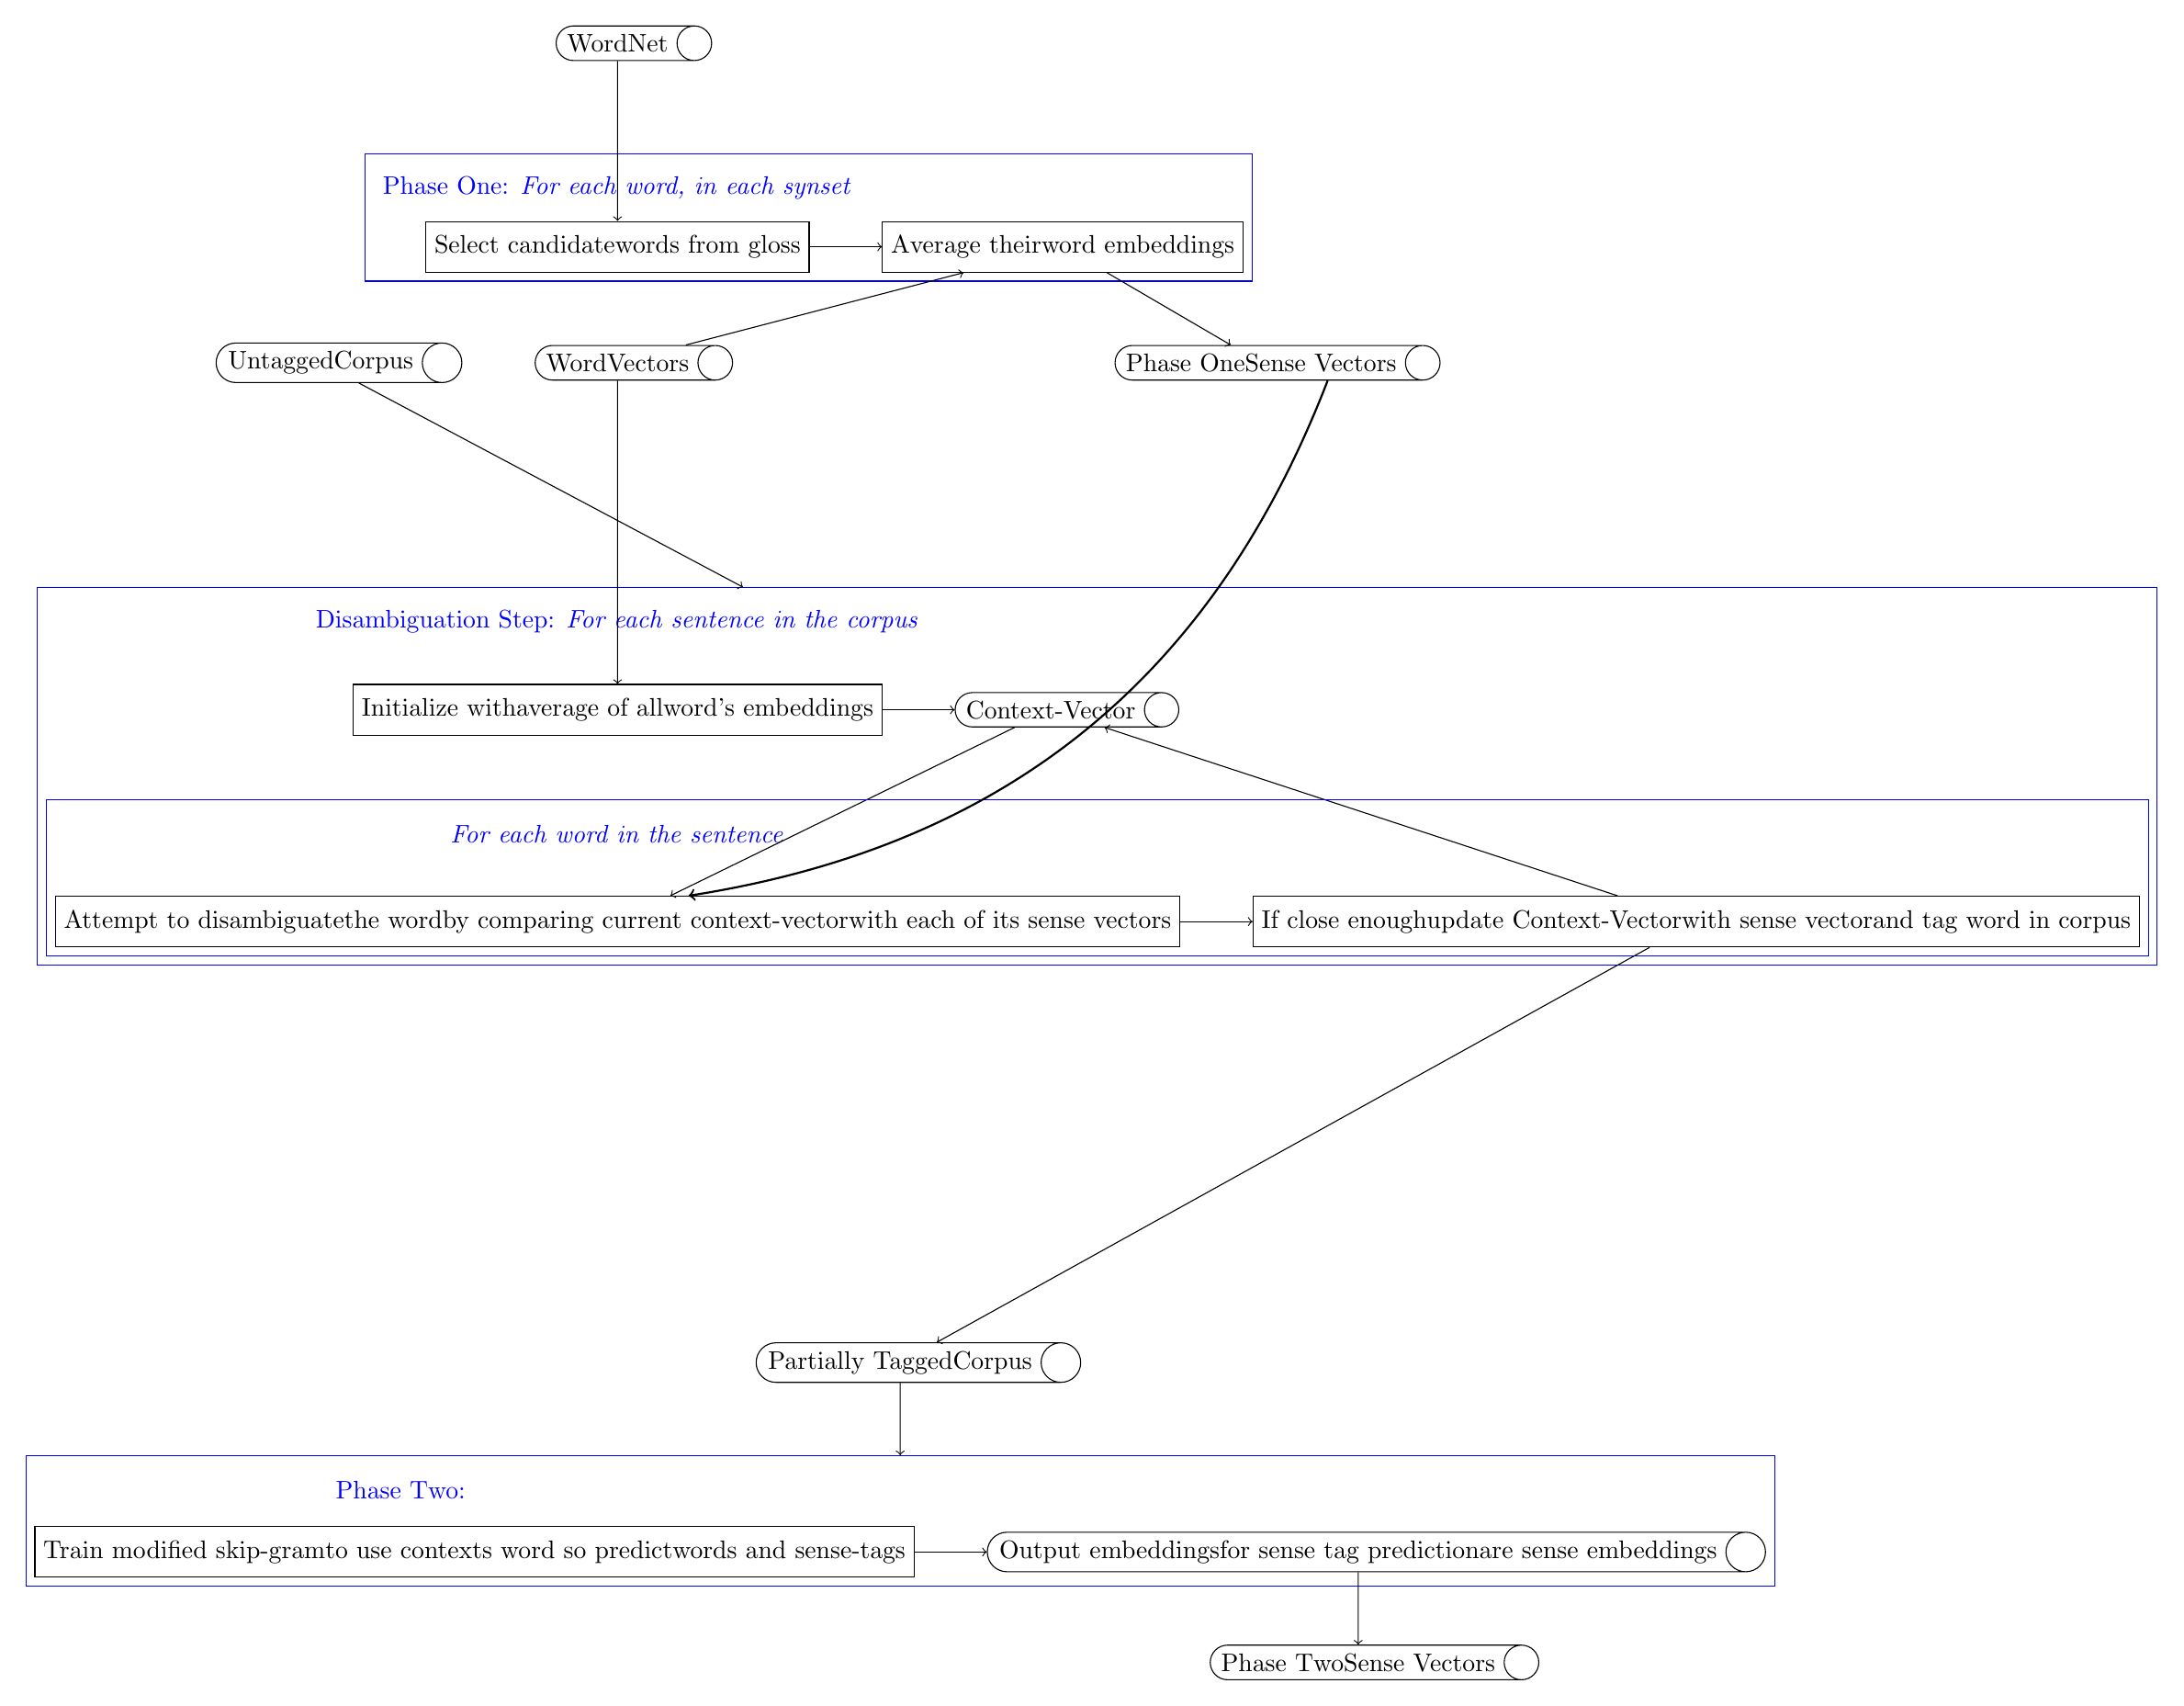
\begin{tikzpicture}
			\node(wordnet)[cylinder,draw]{WordNet};

			\begin{scope}[yshift = -2cm]
				\node(lbl1)[blue]{Phase One: \emph{For each word, in each synset}};
				\node(cands1)[draw, below = 0.1 of lbl1]{Select candidate \\words from gloss};
				\node(average1)[draw, right=of cands1]{Average their\\ word embeddings};
				\draw[->] (cands1) -- (average1);
			\end{scope}
			\node[blue,draw, fit=(lbl1) (average1) (cands1)]{};
			
			\node(wordvecs)[cylinder,draw, below=of cands1] {Word\\Vectors};			
			\node(phaseonevecs)[cylinder, draw, below right=of average1, xshift=-1cm]{Phase One\\ Sense Vectors};
			\draw[->] (wordnet)--(cands1);
			\draw[->] (wordvecs)--(average1);
			\draw[->] (average1)--(phaseonevecs);
			
			\node(corpus)[cylinder, draw, left=of wordvecs]{Untagged\\Corpus};
			
			\begin{scope}[yshift = -8cm]%, xshift=3.2cm]
				\node(lbl2)[blue]{Disambiguation Step: \emph{For each sentence in the corpus}};
				\node(initializecontext)[draw, below=0.5 of lbl2]{Initialize with \\ average of all \\ word's embeddings};
				\node(contextvector)[draw,cylinder, right = of initializecontext]{Context-Vector};

				\draw[->] (initializecontext) -- (contextvector);
				
				\node(lbl2word)[blue, below=of initializecontext]{\emph{For each word in the sentence}};
				\node(disamb)[draw, below=0.5 of lbl2word]{Attempt to disambiguate\\
					the word\\
					 by comparing current context-vector\\ with each of its sense vectors};
				\node(update)[draw, right=of disamb]{If close enough\\ update Context-Vector \\ with sense vector\\and tag word in corpus};
				\draw[->](disamb) --(update);
				\draw[->](contextvector) -- (disamb);
				\draw[->] (update) -- (contextvector);
			\end{scope}
			\node(disambinnerstep)[blue,draw, fit=(lbl2word) (disamb) (update) ]{};
			\node(disambstep)[blue,draw, fit=(initializecontext) (lbl2) (disambinnerstep) ]{};


			
			\draw[->] (wordvecs)--(initializecontext);
			\draw[->] (corpus) -- (disambstep);
			\path[draw, ->, thick] (phaseonevecs.345) to[bend left=30] (disamb.20);
			
			\begin{scope}[yshift = -20cm, xshift=-3cm]
				\node(lbl3)[blue]{Phase Two:};
				\node(cbow)[draw, below = 0.5 of lbl3.east]{Train modified skip-gram \\to use contexts word so predict\\words and sense-tags};
				\node(outputembs)[draw,cylinder, right=of cbow]{Output embeddings\\ for sense tag prediction\\ are sense embeddings};
				\draw[->] (cbow)--(outputembs);
			\end{scope}
			\node(phase2)[blue,draw, fit=(cbow) (lbl3) (outputembs) ]{};
			\node(phasetwovecs)[cylinder, draw, below = of outputembs]{Phase Two\\ Sense Vectors};
			\draw[->] (outputembs)--(phasetwovecs);
						
			\node(taggedcorpus)[cylinder, draw, above = of phase2]{Partially Tagged\\Corpus};
			\draw[->] (update)--(taggedcorpus);
			\draw[->] (taggedcorpus)--(phase2);
		
		\end{tikzpicture}	
	}
\end{figure}

%

The phase one sense vectors have not been assessed on their representational quality.
It could be assumed that because the results for these were not reported, they were worse than those found in phase two.
The phase two sense vectors were not assessed for their capacity to be used for word sense disambiguation.
It would be desirable to extend the method of \textcite{Chen2014}, to use the phase two vectors for WSD.
This would allow this method to be used to disambiguate its own training data,
thus enabling the method to become self-supervised.


\section{Word Sense Induction (WSI)}\label{sec:word sense-induction-wsi}

\aside[Can we go from induced senses to lexical senses]{
	A natural question given the existence of many WSI systems,
	and the existing wealth of lexically indexed resources,
	is if we can align induced senses to a set of lexically defined senses.
	\textcite{agirre2006} proposed a method for doing this using a weighted mapping-based on the probabilities found using induced sense WSD on a labelled ``mapping'' corpus.
	This has only been used on relatively small datasets with only hundreds of words
	(SenseEval 3 \parencite{mihalcea2004senseval} and SemEval-2007 Task 02 \parencite{SemEval2007WSIandWSD}).
	Our own investigations in \textcite{WhiteRefittingSenses} with the larger SemEval 2007 Task 7 \parencite{Navigli:2007:STC:1621474.1621480} suggest that it may not scale very well to to real-word WSD tasks.
	That work proposed an alternative method that worked better, though still not as well as could be hoped.
	Finding suitable methods to link unsupervised representations, to human defined senses remains a topic worthy of research.
}


In this section we will discuss methods for finding a word sense without reference to a standard set of senses.
Such systems must discover the word senses at the same time as they find their representations.
One strong advantage of these methods is that they do not require a labelled dataset.
As discussed there are relatively few high-quality word sense labelled datasets.
The other key advantage of these systems is that they do not rely on fixed senses determined by a lexicographer.
This is particularly useful if the word senses are highly domain specific;
or in a language without strong lexicographical resources.
This allows the data to inform on what word senses exist.

\aside[Why do skip-grams perform so well on SCWS?]{
	SCWS is a corpus designed for evaluating word sense embeddings.
	Single sense embeddings (e.g. skip-grams) cannot take advantage of the context information in the SCWS.
	However, they do often perform comparably to the word sense embeddings.
	Sometimes even outperforming them.
	It is unclear if this highlights the difficulty of the task (i.e. that the impact of context is hard to gauge),
	or it might be due to the (implicit) most frequent sense dominating both the use in the tasks, and the representation in a single sense.
	Alternatively, it may just be the result of the fine tuning of the more mature single-sense embedding methods (and that with more time and tuning multiple sense methods could do proportionally better).
}

Most vector word sense induction and representation approaches are evaluated on similarity tests.
Such tests include WordSim-353 \parencite{WordSim353} for context-less, or Stanford's Contextual Word Similarities (SCWS) for similarity with context information \parencite{Huang2012}.
This evaluation is also suitable for evaluating single sense word-embeddings, e.g. skip-grams.


We can divide the WSI systems into context clustering-based approaches,
and co-location prediction-based approaches.
This division is similar to the separation of co-location matrix factorisation,
and co-location prediction-based approaches discussed in \Cref{sec:word-representations}.
It can be assumed thus that at the core, like for word embeddings,
they are fundamentally very similar.
One could think of prediction of collocated words as a soft indirect clustering of contexts that can have those words.


\subsection{Context Clustering-based Approaches}
As the meaning of a word, according to word embedding principles, is determined by the contexts in which it occurs,
we expect that different meanings (senses) of the same words should occur in different contexts.
If we cluster the contexts that a word occurs in, one would expect to find distinct clusters for each sense of the word.
It is on this principle that the context clustering-based approaches function.



\subsubsection{Offline clustering}\label{sec:offline-clustering}
The fundamental method for most clustering-based approaches is as per \tcite{Schutze:1998wordsenseclustering}.
That original work is not a neural word sense embedding, however the approach remains the same.
\tcite{pantel2002WSI} and \tcite{Reisinger2010} are also not strictly neural word embedding approaches (being more classical vector representations), however the overall method is also very similar.


\aside[On context representations]{
These co-location clustering methods require finding a representation for the context (from this a similarity metric is applied, and the clustering is then done).
More generally, this can be related to the next chapter: \Cref{sec:sentence-representations-and-beyond}, as any of these methods could be used to derive a vector representation of a context.
In most works (including all the works discussed here) comparatively simple representations of the contexts are used.
It would be interesting to extend the sentence representation methods, and apply them to this use.
}

The clustering process is done by considering all word uses, with their contexts.
The contexts can be a fixed-sized window of words (as is done with many word-embedding models), the sentence, or defined using some other rule.
Given a pair of contexts, some method of measuring their similarity must be defined.
In vector representational works, this is ubiquitously done by assigning each context a vector, and then using the cosine similarity between those vectors.

The \textbf{first step} in all the offline clustering methods is thus to define the representations of the contexts.
Different methods define the context vectors differently:
\begin{itemize}
\item \textcite{Schutze:1998wordsenseclustering} uses variations of inverse-document-frequency (idf) weighted bags of words, including applying dimensionality reduction to find a dense representation.
\item \textcite{pantel2002WSI} use the mutual information vectors between words and their contexts.
\item \textcite{Reisinger2010}, use td-idf or $\chi^2$ weighted bag of words.
\item \tcite{Huang2012} uses td-idf weighted averages of (their own) single sense word embeddings for all words in the context.
\item  \tcite{kaageback2015neural} also uses a weighted average of single sense word skip-gram embeddings, with the weighting based on two factors. One based on how close the words were, and the other on how likely the co-occurrence was according to the skip-gram model.

\end{itemize}
It is interesting to note that idf, td-idf, mutual information, skip-gram co-occurrence probabilities (being a proxy for point-wise mutual information \parencite{levy2014neural}), are all closely related measures.

\aside[On clustering]{
	Clustering can be defined as a (mixed integer) optimisation task, of assigning points to clusters so as to satisfy some loss function-based around minimising intra-cluster variance while maximising inter-cluster variance (or a similar measure).
	As this is NP-hard, most clustering methods are approximate.
	K-means is very popular because of its simplicity,
	however it easily falls into local minima,
	and so normally it is run dozens of times (at least) to obtain more optimal results.
	K-means also has the issue of having to select the number of clusters ($k$).
	It should be remembered that there exist many other clustering methods than  k-means (and its variants).
	These other methods use different loss functions, and different strategies to overcome the NP-hard nature of the problem.
	In particular their mixture model methods, hierarchical methods, spectral methods, and others.
	We personally favour affinity propagation \parencite{frey2007clustering},
	though there is provably no ideal clustering algorithm even in the non-heuristic case \parencite{kleinberg2003impossibility}.
	On any clustering task (word sense or otherwise) it is worth investigating several clustering algorithms, and not just settling for k-means (particularly not settling for k-means run once.).
	A series of interesting and easy reading articles on clustering can be found at:
	\url{http://alexhwilliams.info/itsneuronalblog/2015/09/11/clustering1/}, \url{http://alexhwilliams.info/itsneuronalblog/2015/10/01/clustering2/}, and \url{http://alexhwilliams.info/itsneuronalblog/2015/11/18/clustering-is-easy/}
}


The \textbf{second step} in off-line clustering is to apply a clustering method to cluster the word-uses.
This clustering is done based on the calculated similarity of the context representation where the words are used.
Again, different WSI methods use different clustering algorithms.
\begin{itemize}
	\item \textcite{Schutze:1998wordsenseclustering} uses a group average agglomerative clustering method.
	\item \textcite{pantel2002WSI} use a custom hierarchical clustering method.
	\item \textcite{Reisinger2010} use mixtures of von-Mises-Fisher distributions.
	\item \textcite{Huang2012} use spherical k-means.
	\item \textcite{kaageback2015neural} use k-means.
\end{itemize}

The \textbf{final step} is to find a vector representation of each cluster.
For non-neural embedding methods this step is not always done, as defining a representation is not the goal, though in general it can be derived from most clustering techniques.
\textcite{Schutze:1998wordsenseclustering} and 
\textcite{kaageback2015neural} use the centroids of their clusters.
\textcite{Huang2012} use a method of relabelling the word uses with a cluster identifier,
then train a (single-sense) word embedding method on cluster identifiers rather than words.
This relabelling technique is similar to the method later used by \textcite{Chen2014} for learning lexical sense representations, as discussed in \Cref{sec:pseudo-semi-supervised-method}.
As each cluster of contexts represents a sense, those cluster embeddings are thus also considered as  suitable word sense embeddings.

To summarize, all the methods for inducing word sense embeddings via off-line clustering follow the same process.
\textbf{First}: represent the contexts of word use, so as to be able to measure their similarity.
\textbf{Second}: use the context's similarity to cluster them.
\textbf{Finally}: find a vector representation of each cluster.
This cluster representation is the induced sense embedding.

\subsubsection{Online clustering}
The methods discussed above all use off-line clustering.
That is to say the clustering is performed after the embedding is trained.
\tcite{neelakantan2015efficient} perform the clustering during training.
To do this they use a modified skip-gram-based method.
They start with a fixed number of randomly initialised sense vectors for each context.
These sense vectors are used as input embeddings for the skip-gram context prediction task, over single sense output embeddings.
Each sense also has, linked to it, a context cluster centroid, which is the average of all output embeddings for the contexts that the sense is assigned to.
Each time a training instance is presented, the average of the context output embeddings is compared to each sense's context cluster centroid.
The context is assigned to the cluster with the closest centroid, updating the centroid value.
This can be seen as similar to performing a single k-means update step for each training instance.
Optionally, if the closest centroid is further from the context vector than some threshold,  a new sense can be created using that context vector as the initial centroid.
After the assignment of the context to a cluster, the corresponding sense vector is selected for use as the input vector in the skip-gram context prediction task.

\textcite{kaageback2015neural} investigated using their weighting function (as discussed in \Cref{sec:offline-clustering}) with the online clustering used by \textcite{neelakantan2015efficient}.
They found that this improved the quality of the representations.
More generally any such weighting function could be used.
This online clustering approach is loosely similar to the co-location prediction-based approaches.


\subsection{Co-location Prediction-based Approaches}
\aside[Probability]{
One may wish to brush up on basic probability notions for this section.
In particular joint, conditional and marginal probabilities definitions;
as well as Bayes Theorem and the probability chain-rule which come from those.
In brief these are as follows.

\smallskip
\textbf{Conditional Probability:}
\mbox{$P(A\mid B)=\frac{P(A, B)}{P(B)}$}

\smallskip
\textbf{Marginal Probability:}
\mbox{$P(A)=\sum_{\forall b} P(A, B=b)$}

\smallskip
\textbf{Bayes Theorem:}
\mbox{$P(A\mid B)=\frac{P(B \mid A)P(A)}{P(B)}$}

\smallskip
\textbf{Probability Chain-rule}:
\mbox{$P(\n A_n,\ldots,\n A_1)$}\\
\resizebox{\notescolwidth}{!}{$\quad=P(\n A_n\mid \n A_{n-1},\ldots,\n A_1)P(\n A_{n-1},\ldots,\n A_1)$}
e.g.
\mbox{$P(A,B,C)$}
\mbox{$\quad=P(A\mid B,C) P(B \mid C) P(C)$}
\smallskip
The latter three rules are consequences of the first.
}
Rather than clustering the contexts, and using those clusters to determine embeddings for different senses, one could consider the sense as a latent variable in the task used to find word embeddings -- normally a language modelling task.
The principle is that it is not the word that determines its collocated context words,
but rather the word sense.
So the word sense can be modelled as a hidden variable, where the word, and the context words are being observed.



\tcite{tian2014probabilistic} used this to define a  skip-gram-based method for word sense embeddings.
For input word $\n w_i$ with  senses $\seq S(\n w_i)$,
the probability of output word $\n w_o$ occurring near $\n w_i$ can be given as:
\begin{equation}
	P(\n w_o\mid \n w_i) = \sum_{\forall \n s_k \in \seq S(\n w_i)} P(\n w_o \mid \n s_k, \n w_i) P(\n s_k \mid \n w_i) \label{equ:tianmm}
\end{equation}

Given that a sense $\n s_k$ only belongs to one word $\n w_i$,
we know that $k$th sense of the $i$th word only occurs when the $i$th word occurs.
We have that the join probability $P(\n w_i,\n s_k) = P(\n s_k)$.
%and $P(\n w_i) = \sum_{\forall \n s_k \in \seq S(\n w_i) P(\n s_k)}$;

We can thus rewrite \Cref{equ:tianmm} as:
\begin{align}
P(\n w_o\mid \n w_i) &= \sum_{\forall \n s_k \in \seq S(\n w_i)} P(\n w_o \mid \n s_k) \, P(\n s_k \mid \n w_i) \label{equ:tianmm2}
\end{align}

A softmax classifier can be used to define $P(\n w_o \mid \n s_k)$, just like in normal language modelling.
With output embeddings for the words $\n w_o$, and input embeddings for the word senses $\n s_k$.
This softmax can be sped-up using negative sampling or hierarchical softmax.
The later was done by \textcite{tian2014probabilistic}.

\Cref{equ:tianmm2} is in the form of a mixture model with a latent variable.
Such a class of problems are often solved using the Expectation Maximisation (EM) method.
In short, the EM procedure functions by performing two alternating steps.
The \textbf{E-step} calculates the expected chance of assigning word sense for each training case ($\hat{P}(\n s_l \mid \n w_o)$) in the training set $\seq X$.
Where a training case is a pairing of a word use $\n w_i$, and context word $\n w_o$, with $\n s_l\in \seq S(\n w_i)$, formally we have:
\begin{align}
\hat{P}(\n s_l \mid \n w_o) = \frac{\hat{P}(\n s_l \mid \n w_i) P(\n w_o \mid \n s_l)}{\sum_{\forall \n s_k \in \seq S(\n w_i)} \hat{P}(\n w_o \mid \n s_k) P(\n s_k \mid \n w_i)}
\end{align}

The \textbf{M-step} updates the prior likelihood of each sense (that is without context) using the expected assignments from the E-step.

\begin{align}
\hat{P}(\n s_l \mid \n w_i) = \frac{1}{\left|\seq X\right|} \sum_{\forall (\n w_o,\n w_i)\in \seq X} \hat{P}(\n s_l \mid \n w_o)
\end{align}

During this step the likelihood of the $P(\n w_o \mid \n w_i)$ can be optimised to maximise the likelihood of the observations.
This is done via gradient descent on the neural network parameters of the softmax component: \mbox{$P(\n w_o \mid \n s_k)$}.
By using this EM optimisation the network can fit values for the embeddings in that softmax component.


A limitation of the method used by \textcite{tian2014probabilistic}, is that the number of each sense must be known in advance.
One could attempt to solve this by using, for example, the number of senses assigned by a lexicographical resource (e.g. WordNet).
However, situations where such resources are not available or not suitable are one of the main circumstances in which WSI is desirable  (for example in work using domain specific terminology, or under-resourced languages).
In these cases one could apply a heuristic-based on the distribution of senses-based on the distribution of words \parencite{zipf1945meaning}.
An attractive alternative would be to allow senses to be determined-based on how the words are used. If they are used in two different ways, then they should have two different senses.
How a word is being used can be determined by the contexts in which it appears.


\tcite{AdaGrams} extend on this work by making the number of senses for each word itself a fit-able parameter of the model.
This is a rather Bayesian modelling approach, where one considers the distribution of the prior.


\aside[WordNet and BabelNet]{
	As mentioned in the previous sections, WordNet and BabelNet are the predominant lexicons used for word senses. It is not directly relevant to this section, but we have space here to remark upon them.
	WordNet \parencite{tengi1998design} as a very well established tool has a have a binding in practically every modern programming language suitable for NLP.
	WordNet.jl (\url{https://github.com/JuliaText/WordNet.jl}) is the Julia binding.
	NLTK \parencite{bird2009natural} includes one for Python.
	
	BabelNet \parencite{navigli2010babelnet} is intended to be accessed as an online resource, via a RESTful API. Users receive 1000 free queries per day.
	Academic users can request an upgrade to 50,000 queries per day, or to download a copy of the database.
	From personal experience we found those requests to be handled easily and rapidly.
}


Considering again the form of \Cref{equ:tianmm2}
\begin{align}
P(\n w_o\mid \n w_i) &= \sum_{\forall \n s_k \in \seq S(\n w_i)} P(\n w_o \mid \n s_k) P(\n s_k \mid \n w_i) 
\end{align}
The prior probability of a sense given a word, but no context, is 
$P(\n s_k \mid \n w_i)$.
This is Dirichlet distributed.
This comes from the definition of the Dirichlet distribution as the the prior probability of any categorical classification task.
When considering that the sense my be one from an unlimited collection of possible senses,
then that prior becomes a Dirichlet process.

In essence, this prior over a potentially unlimited number of possible senses becomes another parameter of the model (along with the input sense embeddings and output word embeddings).
The fitting of the parameters of such a model is beyond the scope of this book;
it is not entirely dissimilar to the fitting via expectation maximisation incorporating gradient descent used by  \textcite{tian2014probabilistic}.
The final output of \textcite{AdaGrams} is as desired:
a set of induced sense embeddings, 
and a language model that is able to predict how likely a word is to occur near that word sense ($P(\n w_o \mid \n s_k)$).

By application of Bayes' theorem, the sense language model can be inverted to take a word's context,
and predict the probability of each word sense.

\aside[Independence Assumption]{Technically, \Cref{equ:bayeswds} does not require the independence of the probabilities of the context words.
Rather it only requires that the context words be conditionally independent on the word in question $\n w_i$.
Nevertheless, even the conditional independence assumption is incorrect, except for a theoretical perfect embedding capturing perfect information.
The conditional independence assumption remains useful as an approximation.
}

\begin{equation}
P(\n s_l \mid \n w_o) = \frac{P(\n w_o \mid \n s_l) P(\n s_l \mid \n w_i)}{\sum_{\forall \n s_k \in \seq S(\n w_i)} P(\n w_o \mid \n s_k) P(\n s_k \mid \n w_i)} \label{equ:bayeswds}
\end{equation}
with the common (but technically incorrect) assumption that all words in the context are independent. 


\aside[Finding the nearest neighbours (Nearest Neighbour Trees)]{
	A common evaluation task with any representation (once trained) is to find its nearest neighbours, given a particular point.
	The na\"ive solution is to check the distance to all points.
	For $n$ points this is $O(n)$ operations.
	For word embeddings $n$ is the size of the vocabulary, perhaps $100,000$ words.
	Performing $100,000$ operations per check, is not entirely unreasonable on modern computers (even when the operations are on 300 dimensional representations).
	However, for word sense embeddings, which have many senses per word in the vocabulary,
	this means many more points to check.
	30 senses per word is not unusual for fine-grained word sense induction.
	Having a total $n=3,000,000$ representations to check causes a noticeable delay.
	To solve this we can use  data structures designed for fast nearest neighbour querying.
	A k-d tree  takes at worst $O(n \log_2(n))$ time to construct.
	Once constructed on average it takes $O(\log (n))$ to find the nearest neighbour to any point.
	This makes checking the nearest neighbour nearly instantaneous for even the largest vocabularies.
}

Given a context window:\\
 $\n \seq{W}_i = \left( \n w_{i-\frac{n}{2}},\ldots, \n w_{i-1}, \n w_{i+1},\ldots, \n w_{i+\frac{n}{2}}\right)$,
we have:
\begin{equation}
P(\n s_l \mid \n \seq{W}_i) = 
\frac{\prod_{\forall \n w_{j}\in \n \seq{W}_i} P(\n w_{j} \mid \n s_l) P(\n s_l | \n w_i)}{\sum_{\n s_k \in \seq S(\n w_i)} \prod_{\forall \n w_{j} \in \n \seq{W}_i} P(\n w_{j} \mid \n s_k) P(\n s_k | \n w_i)}
\end{equation}



\section{Conclusion}

Word sense representations allow the representations of the senses of words when one word has multiple meanings.
This increases the expressiveness of the representation.
These representations can in general be applied anywhere word embeddings can.
They are particularly useful for translation,
and in languages with large numbers of homonyms.

The word representation discussions in this chapter naturally lead to the next section on phrase representation. Rather than a single word having many meanings, the next chapter will discuss how a single meaning may take multiple words to express.
In such longer structure's representations, the sense embeddings discussed here are often unnecessary,
as the ambiguity may be resolved by the longer structure.
Indeed, the methods discussed in this chapter have relied on that fact to distinguish the senses using the contexts.


\end{document}